\subsection{Network Design}

\begin{figure*}[t]
    \centering
    \begin{subfigure}{0.4\textwidth}
        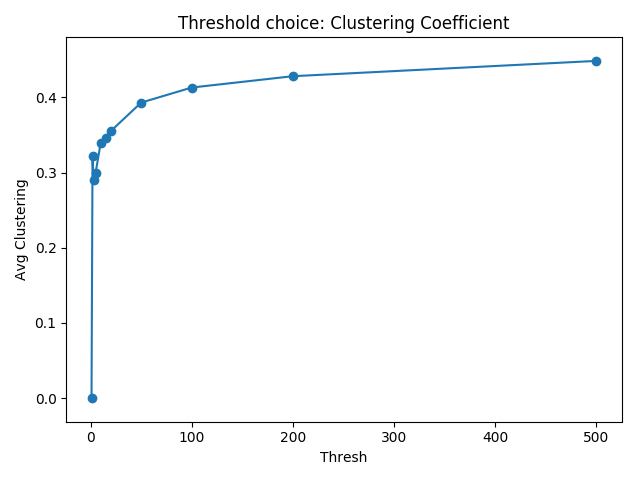
\includegraphics[width=1.\textwidth]{images/thresh_vs_avg_clustering.png}
        \caption{Clustering Coefficient vs. Threshold Size}
    \end{subfigure}
    ~
    \begin{subfigure}{0.4\textwidth}
        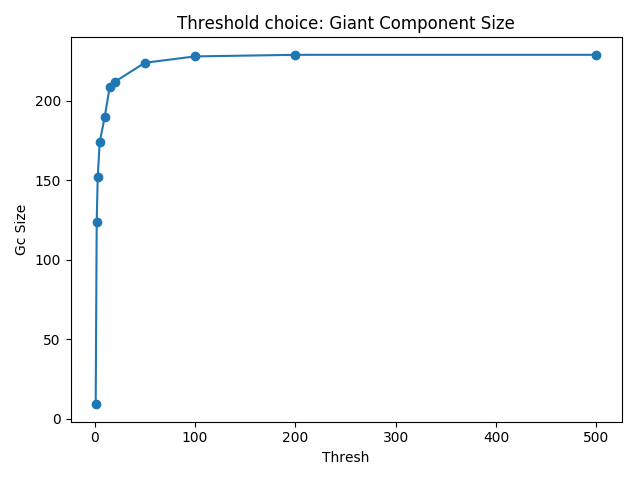
\includegraphics[width=1.\textwidth]{images/thresh_vs_gc_size.png}
        \caption{Giant Component Size vs. Threshold Size}
    \end{subfigure}
    \caption{Comparing threshold size effect on clustering coefficient and giant component size in order to determine the ideal threshold size.}
    \label{fig-threshold-size}
\end{figure*}

\subsubsection{Nodes and Edges}
Network nodes constitute each character identified in the set of found named entities. These were referenced against online resources to ensure proper coverage of the characters in the book. Edges in the book represent a co-mention between two entities in the text.

A threshold number of tokens (words) under which the number of tokens between the mention of one entity and another determines if an edge is established. If the edge already exists, the weight is updated. The current entity $i$ is only matched with proceeding entities $j$ within this threshold. Once no match is found, the next available entity is checked for proceeding matches.

The threshold number of tokens is determined by a semi-objective measure of the effect of the threshold length on the average clustering coefficient and the giant component size (see Figure \ref{fig-threshold-size}). The intuition behind the use of these metrics is that we choose the minimum threhold length required to produce a large giant component and ample enough clustering best capturing the highly connected nature of characters in the novel. Our chosen threshold is 50 tokens.

